\documentclass[a4paper,10pt]{article}
\usepackage{mathtext}
\usepackage[T2A]{fontenc}
\usepackage[utf8]{inputenc}
\usepackage[russian]{babel}
\usepackage{amsmath}
\usepackage{amsfonts}
\usepackage{amssymb}
\usepackage{graphicx}
\usepackage[left=2cm,right=2cm,
    top=2cm,bottom=2cm,bindingoffset=0cm]{geometry}
\usepackage{color}
\usepackage{gensymb}

\usepackage{enumitem}
\setlist[enumerate]{label*=\arabic*.}

\usepackage{indentfirst}

\usepackage{titlesec}
\newcommand{\sectionbreak}{\clearpage}

%\graphicspath{ {<GraphicsPath>/} }
 
\begin{document}
\begin{titlepage}
  \begin{center}
    МОСКОВСКИЙ ГОСУДАРСТВЕННЫЙ УНИВЕРСИТЕТ \\ ИМ. Н.Э.БАУМАНА
    \vspace{0.25cm}
    
    Факультет "Энергомашиностроение"
    
    Кафедра "Э3"
    \vfill
    
    
    Жигалкин Александр Сергеевич
    \vfill

    \textsc{Курсовоей проект}\\[5mm]
    
    {\LARGE Проектирование свободной турбины ТВлД}
\end{center}
\vfill

\newlength{\ML}
\settowidth{\ML}{«\underline{\hspace{0.7cm}}» \underline{\hspace{2cm}}}
\hfill\begin{minipage}{0.4\textwidth}
  Руководитель курсового проекта\\
  \underline{\hspace{\ML}} В.\,Н.~Шадрин\\
  «\underline{\hspace{0.7cm}}» \underline{\hspace{2cm}} 2016 г.
\end{minipage}%
\bigskip

\vfill

\begin{center}
  Москва, 2016 г.
\end{center}
\end{titlepage}

\section{Задание}

Спроектировать двуступенчатую свободную турбину турбовального двигателя c температурой после камеры сгорания $T_г^*=1463\ К$ и мощностью на валу свободной турбины $N_e=2.07\ МВт$. 

\begin{figure}[hbtp]
\centering
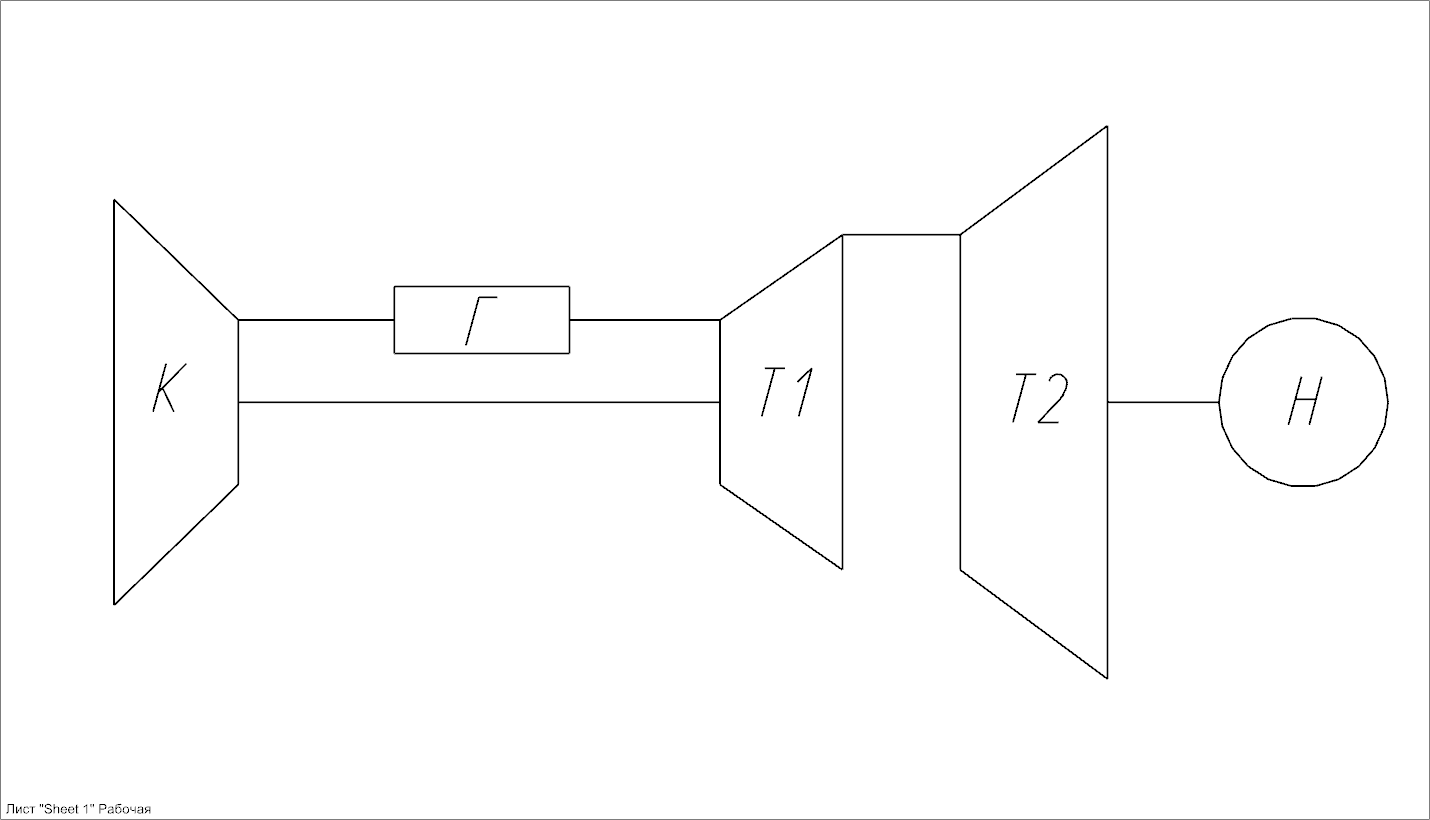
\includegraphics[scale=0.2]{../scheme.png}
\caption{Схема ГТД}
\end{figure}



\tableofcontents
\newpage

\section{Расчет параметров цикла ГТД}

\subsection{Исходные данные}
\begin{center}
	\begin{tabular}{|p{7cm}|c|c|c|}
		\hline
		\textbf{Величина} & \textbf{Обозначение} & \textbf{Размерность} & \textbf{Значение} \\ \hline
		Политропический КПД компрессора & $\eta_{кp}^*$ & - & 0.9 \\ \hline
		Полнота сгорания топлива & $\eta_г$ & - & 0.98 \\ \hline
		Политропический КПД турбины компрессора & $\eta_{ткp}^*$ & - & 0.91 \\ \hline
		Политропический КПД свободной турбины & $\eta_{тp}^*$ & - & 0.91 \\ \hline
		Относительная скорость на выходе из ГТД & $\lambda_{вых}$ & - & 0.05 \\ \hline
		Мощность на валу свободной турбины & $N_e$ & кВт & 2069.0 \\ \hline
		Температура перед турбиной компрессора & $T_г^*$ & К & 1463.5 \\ \hline
		Коэффициент сохранения полного давления во входном устройстве компрессора & $\sigma_{вх}$ & - & 0.995 \\ \hline
		Коэффициент сохранения полного давления в камере сгорания & $\sigma_{г}$ & - & 0.961 \\ \hline
		Коэффициент сохранения полного давления в выходном патрубке & $\sigma_{вых}$ & - & 0.995 \\ \hline
		Механический КПД турбины компрессора & $\eta_м$ & - & 0.99 \\ \hline
		КПД редуктора & $\eta_р$ &  - & 0.985 \\ \hline
		Относительный расход утечек & $g_{ут}$ &  - &0.01 \\ \hline
		Относительный расход на охлаждение & $g_{охл}$ &  - & 0.18 \\ \hline
		Относительный расход возвращаемого воздуха & $g_{возвр}$ & - & 0.02 \\ \hline
	\end{tabular}
\end{center}

\subsection{Вариантные расчеты}
Для определения оптимальной степени повышения давления в компрессоре был произведен расчет цикла ГТД для различных значений  $\pi_к^*$ в интервале 6 до 27. В результате были построены графики зависимостей КПД, удельной расхода топлива и расхода через компрессор от степени повышения давления в компрессоре.

Ниже представлены графики зависимостей КПД, расхода топлива и расхода воздуха ГТД от $\pi_к^*$. Также представлен их сводный график, на котором для наглядности значения КПД, расхода топлива и расхода воздуха отнесены к максимальным на представленном промежутке значений степени повышения давления.

\begin{center}


	\begin{figure}[hbtp] \centering 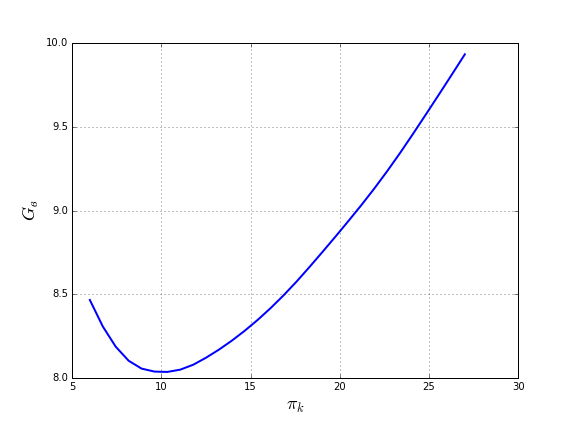
\includegraphics[scale=0.5] {../../plots/cycle_G_air.png} \caption{Зависимость расхода воздуха от степени повышения давления} \end{figure}	
	
	\begin{figure}[hbtp] \centering 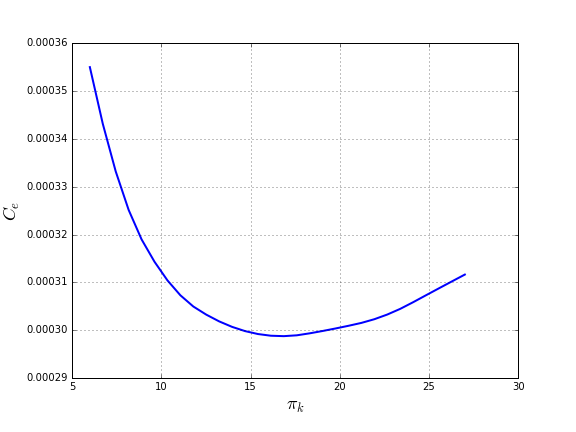
\includegraphics[scale=0.5] {../../plots/cycle_C_e.png} \caption{Зависимость удельного расхода топлива от степени повышения давления} \end{figure}
	 
	\begin{figure}[hbtp] \centering 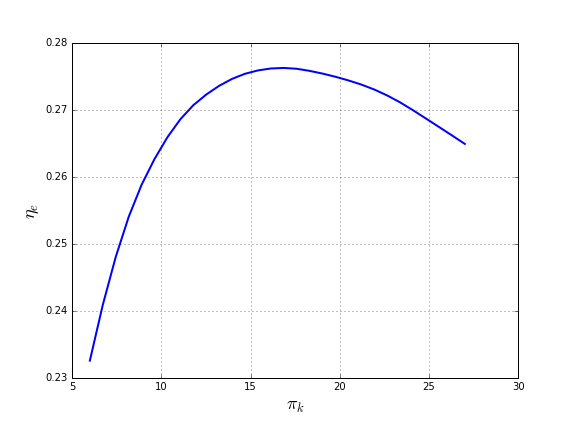
\includegraphics[scale=0.5] {../../plots/cycle_eta_e.png} \caption{Зависимость КПД двигателя от степени повышения давления} \end{figure} 
\end{center}

\begin{figure}[hbtp]
\centering
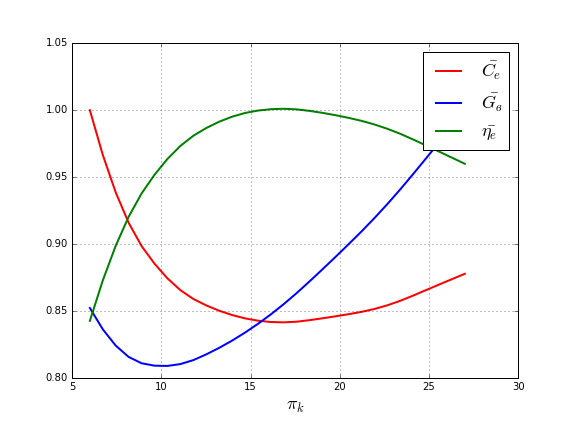
\includegraphics[scale=0.5]{../../plots/cycle_relative_quantities.png}
\caption{Сводный график зависимостей КПД, расхода воздуха и расхода топлива от степени повышения давления в компрессоре}
\end{figure}



В качестве оптимального принимаем $\pi_к = 13.41$.

Ниже представлен расчет цикла ГТД при $\pi_к = 13.41$

\subsection{Расчет цикла при $\pi_к = 13.41$}
Расчет некоторых узлов ГТД (а именно обоих турбин и компрессора) носит итерационный характер, так как удельная теплоемкость и коэффициент адиабаты зависят от температуры на выходе из узла. Поэтому ниже представлены расчеты для последних итераций.
\begin{enumerate}
	\item Определим давление за входным устройством: $$p_{вх}^* = \sigma_{вх} p_{а} = 0.995 \cdot 0.1013 = 0.101 \/\ МПа$$
	\item Определим давление за компрессором: $$p_к^* = \pi_к p_{вх}^* = 13.41 \cdot 0.101 = 1.352 \/\ МПа$$
	\item Определим адиабатический КПД компрессора, принимая показатель адиабаты воздуха $k_в = 1.403$: 
	\[\eta_{к}^* = \frac{\pi_к^{\frac{k_в - 1}{k_в} - 1}}
						{\pi_к^{\frac{k_в - 1}{k_в \eta_{кp}^* - 1}}} = 
		\frac{13.41^{\frac{1.403 - 1}{1.403} - 1}}
						{13.41^{\frac{1.403 - 1}{1.403 \cdot 0.9 - 1}}} = 0.8589\]
	\item Определим температуру газа за компрессором: 
	$$T_к^* = T_a \left[ 1 + \frac{\pi_к^{\frac{k_в - 1}{k_в}} - 1}{\eta_к^*} \right] = 
	288 \left[ 1 + \frac{{13.41}^{\frac{1.403 - 1}{1.403}} - 1}{0.8589} \right] = 659.096 \/\ К$$
	\item Определим уточненное значение показателя адиабаты:
	\begin{enumerate}
	
	\item Средняя теплоемкость воздуха при температуре $T_a$:
	\[c_{pв ср}(T_a) = \left( 1.2 \cdot 10^{-5} \left( T_a - 70 \right) + 0.236 \right) \cdot 4.187 \cdot 10^3 = \] 
	\[=\left( 1.2 \cdot 10^{-5} \left( 288 - 70 \right) + 0.236 \right) \cdot 4.187 \cdot 10^3 =  999.085\ Дж / (кг \cdot К)
	\]
	\item Средняя теплоемкость воздуха при температуре $T_к^*$:
	\[c_{pв ср}(T_к^*) = \left( 1.2 \cdot 10^{-5} \left( T_a - 70 \right) + 0.236 \right) \cdot 4.187 \cdot 10^3 = \]
	\[=\left( 1.2 \cdot 10^{-5} \left( 659.096 - 70 \right) + 0.236 \right) \cdot 4.187 \cdot 10^3 =  1017.731\ Дж / (кг \cdot К)\]
	\item Cредняя теплоемкость воздуха в интервале температур от $T_a$ до $T_к^*$:
	\[c_{pв} = \frac{
	c_{pв ср}(T_к^*) (T_к^* - T_0) - c_{pв ср}(T_a)(T_a - T_0)
	}{
	T_к^* - T_a} = \]
	\[ =\frac{
	1017.731 \cdot (659.096 - 273) - 999.085 \cdot (288 - 273)
	}{
	659.096 - 288} = 1018.484\ Дж / (кг \cdot К)\]
	
	\item Новое значение показателя адиабаты:
	\[k_в^\prime = \frac{c_{pв}^\prime}{c_{pв}^\prime - R_в} = \frac{1018.484}{1018.484 - 287.4} = 1.393\]
	\end{enumerate}
	
	\item Определим погрешность определения показателя адиабаты:
	$$\delta = \frac{\left| k_в^\prime - k_в \right|}{k_в} \cdot 100 \% = 
	\frac{\left| 1.393 - 1.403 \right|}{1.403} \cdot 100 \% = 
	0.68 \% < 5 \%$$
	Точность определения показателя адиабаты воздуха находится в пределах допуска.
	\item Используя найденный показатель адиабаты воздуха, определим теплоемкость воздуха в процессе сжатия воздуха в компрессоре:
	$$c_{pв} = \frac{k_в}{k_в - 1} R_в = 
	\frac{1.403}{1.403 - 1} \cdot 287.4 = 
	1018.484 \/\ Дж/кг$$
	\item Определим работу компрессора:
	$$L_к = c_{pв} \left( T_к^* - T_a \right) = 
	1018.484 \cdot \left( 659.096 - 288 \right) = 
	0.378 \cdot 10^6 \/\ Дж/кг $$
	\item Температура газа за камерой сгорания:
	$$T_г^* = 1463.5 \/\ К$$
	\item Определим относительный расход топлива. Теплоемкость продуктов сгорания керосина рассчитывается через коэффициент избытка воздуха температуру. При расчета приняты следующие значения: 
	\begin{enumerate} % список значений для расчета удельного расхода топлива
		
		\item[1)] температура определения теплофизических параметров веществ: 
		$$T_0 = 290 \/\ К;$$
		\item[2)] средняя теплоемкость воздуха перед камерой сгорания: 
		$$c_{pв}\left( T_к^* \right) = 1017.731 \/\ Дж/(кг \cdot К);$$
		\item[3)] средняя теплоемкость чистых продуктов сгорания керосина после камеры сгорания: 
		\[c_{pг}\left( T_г^*,\ 1 \right) = \left[
		\frac{1.25 + 2.2}{10^5} (T_г^* + 450) + 0.218 
		\right]\cdot 4.187 \cdot 10^3 = \]
		\[=\left[
		\frac{1.25 + 2.2}{10^5} (1463.5 + 450) + 0.218 
		\right]\cdot 4.187 \cdot 10^3 = 1189.174 \/\ Дж/(кг \cdot К);\]
		\item[4)] средняя теплоемкость чистых продуктов сгорания керосина при температуре $T_0$: 
		\[c_{pг}\left( T_0,\ 1 \right) = \left[
		\frac{2.25 + 1.2}{10^5} (T_0 - 70) + 0.236 \right] \cdot 4.187 \cdot 10^3 = \]
		\[\left[
		\frac{2.25 + 1.2}{10^5} (290 - 70) + 0.236 \right] \cdot 4.187 \cdot 10^3 = 
		1019.622 \/\ Дж/(кг \cdot К);\]
		\item[5)] низшая теплота сгорания топлива: $$Q_н^р = 43600.0 \cdot 10^3 \/\ Дж / (кг \cdot К);$$
		\item[6)] полнота сгорания: $$\eta_г = 0.98;$$
		\item[7)] масса воздуха, необходимая для сжигания 1 кг топлива:
		$$l_0 = 14.61 \/\ кг;$$
	\end{enumerate}

	\begin{enumerate}
		
		\item Определим относительный расход топлива:
		
		\[g_m = \frac{G_m}{G_в^г} = 
		\frac{
			c_{pг} \left( T_г^* \right) T_г^* - 
			c_{pв} \left( T_к^* \right) T_к^* 
		}{
			Q_н^р \eta_г - 
			\left[
				c_{pг} \left( T_г^* \right) T_г^* - 
				c_{pг} \left( T_0 \right) T_0 \right]	} =  \]
		\[=
		\frac{
			1189.174 \cdot 1463.5 - 
			1017.731 \cdot 659.096 
		}{
			43600.0 \cdot 10^3 \cdot 0.98 - 
			\left[
				1189.174 \cdot 1463.5 - 
				1019.622 \cdot 290
			\right]		
		} = 0.0259\]
		
		\item Определим коэффициент избытка воздуха:
		$$\alpha = \frac{1}{g_m l_0} = 
		\frac{1}{0.0259 \cdot 14.61} = 2.642$$	
	\end{enumerate}
	
	\item Определим относительный расход газа:
		$$g_{г} = \left( 1 + g_m \right) \left( 1 - g_{ут} - g_{охл} \right) + g_{возвр} = 
		\left( 1 + 0.0259 \right) \left( 1 - 0.01 - 0.18 \right) + 0.02 = 0.851$$
Расчет турбины компрессора состоит из двух частей. Первая часть - это определения температуры на выходе из турбины. Этот расчет является итерационным и ведется до сходимости по $k_г$.  Вторая часть - расчет давления торможения на выходе из турбины. Этот расчет также является итерационным и ведется до сходимости по $\pi_{тк}^*$. Ниже приведены последнии итерации обоих расчетов.	
	\item Определим удельную работу турбины компрессора:
	$$L_{тк} = \frac{L_к}{g_{г}\eta_м} = \frac{0.378 \cdot 10^6}{0.851 \cdot 0.99 } = 0.449 \cdot 10^6 \/\ Дж/кг$$
	\item Определим давление газа перед турбиной компрессора:
	$$p_г^* = p_{к}^* \sigma_г = 1.352 \cdot 0.961 = 1.299 \/\ МПа$$
	\item Определим среднюю теплоемкость газа в процессе расширения газа в турбине, принимая показатель адиабаты газа $k_г = 1.309$:
	$$c_{pг} = \frac{k_г}{k_г - 1} R_г = 
	\frac{1.309}{1.309 - 1} \cdot 287.4 = 1218.599 \/\ Дж/(кг \cdot К) $$
	\item Определим температуру за турбиной компрессора:
	\[T_{тк}^* = T_г^* - \frac{L_{тк}}{c_{pг}} =
	1463.5 - \frac{0.449 \cdot 10^6}{1218.599} = 1095.352\]

	\item Определим уточненное значение показателя адиабаты газа:
	
	\begin{enumerate}
	\item Определим значение средней теплоемкости газа при температуре $T_{тк}^*$:
	\[c_{pг\ ср}(T_{тк}^*) = \left[ 
	\frac{1.25 +2.2 \alpha}{\alpha \cdot 10^5} (T_{тк}^* + 450) + 0.218
	\right] \cdot 4.187 \cdot 10^3= \]
	\[=\left[ 
	\frac{1.25 +2.2 \cdot 2.642}{2.642 \cdot 10^5} (1095.352 + 450) + 0.218
	\right] \cdot 4.187 \cdot 10^3= 1085.731\ Дж / (кг \cdot К) \]
	\item Определим значение средней теплоемкости при температуре $T_г^*$:
	\[c_{pг\ ср}(T_г^*) = \left[ 
	\frac{1.25 +2.2 \alpha}{\alpha \cdot 10^5} (T_{тк}^* + 450) + 0.218
	\right] \cdot 4.187 \cdot 10^3= \]
	\[\left[ 
	\frac{1.25 +2.2 \cdot 2.642}{2.642 \cdot 10^5} (1095.352 + 450) + 0.218
	\right] \cdot 4.187 \cdot 10^3= 1006.859\ Дж / (кг \cdot К) \]
	\item Новое значение средней теплоемкости в интервале температур от $T_{тк}^*$ до $T_г^*$:
	\[c_{pг}^\prime = \frac{
	c_{pг\ ср}(T_г^*) (T_г^* - T_0) - c_{pг\ ср}(T_{тк}^*)(T_{тк}^* - T_0)
	}{
	T_{г}^* - T_{тк}^*} = \]
	\[=\frac{
	1006.859 \cdot (1463.5 - 273) - 1085.731 \cdot (1095.352 - 273)
	}{
	1463.5 - 1095.352} = 1218.978\ Дж / (кг \cdot К)\]
	\item Новое значение показателя адиабаты:
	\[k_в^\prime = \frac{c_{pг}^\prime}{c_{pг}^\prime - R_г} = \frac{1218.978}{1218.978 - 287.4} = 1.309\]
	\end{enumerate}

	\item Определим погрешность определения показателя адиабаты:
	$$\delta = \frac{\left| k_г^\prime - k_г \right|}{k_г} \cdot 100 \% = 
	\frac{\left| 1.309 - 1.309 \right|}{1.309} \cdot 100 \% = 
	0.01 \% < 5 \%$$
	Погрешность определения показателя адиабаты в пределах допуска.
	\item Определим значение адиабатического КПД турбины компрессора, приняв степень понижения давления $\pi_{тк} = 3.872$:
	\[\eta_{тк}^* = \frac{1 - \pi_{тк} ^ 
	                   {\frac{\left(1 - k_г \right) \eta_{ткp}^*}{k_г}}}
	              {1 - \pi_{тк} ^ 
	                   {\frac{1 - k_г}{k_г}} } = 
	          \frac{1 - 3.872 ^ 
	                   {\frac{\left(1 - 1.309 \right) \cdot 0.91}{1.309}}}
	              {1 - 3.872 ^ 
	                   {\frac{1 - 1.309}{1.309}} } = 0.922 \]	
	\item Определим давление воздуха за турбиной компрессора:
	$$p_{тк}^* = p_г^* 
	\left[ 
		1 - \frac{L_{тк}}{c_{pг} T_г^* \eta_{тк}^*}	
	\right] ^ \frac{k_г}{k_г - 1} = 	
	1.299 
	\left[ 
		1 - \frac{0.449 \cdot 10^6}
		{1218.599 \cdot 1463.5 \cdot 0.922}	
	\right] ^ \frac{1.309}{1.309 - 1} =
	 0.337 \/\ МПа$$
	 \item Определим новую степень понижения давления:
	 \[\pi_{тк}^{*\prime} = \frac{p_г^*}{p_{тк}^*} = \frac{1.299}{0.337} = 3.857\]
	 \item Определим погрешность определения степени понижения давления:
	 $$\delta = \frac{\left| \pi_{тк}^{*\prime} - \pi_{тк}^* \right|}{\pi_{тк}^*} \cdot 100 \% = 
	\frac{\left| 3.857 - 3.872 \right|}{3.872} \cdot 100 \% = 
	0.39 \% < 5 \%$$
	Погрешность определения степени понижения давления в пределах допуска.
	
	
	\item Зададим значение приведенной скорости на выходе из выходного устройства:
	$$\lambda_{вых} = 0.05$$
	\item Определим давление торможения на выходе из выходного устройства, задавая показатель адиабаты газа $k_г = 1.321$:
	$$p_{вых}^* = p_a \pi \left( \lambda_{вых}, k_г \right) = 
	0.1013 \cdot \pi \left( 0.05, 1.321 \right) = 
	0.101 \/\ МПа$$

	\item Определим давление торможения за силовой турбиной:
	$$p_т^* = \frac{p_{вых}^*}{\sigma_{вых}} = \frac{0.101}{0.995} = 
	0.102 \/\ МПа$$
	\item Определим степень понижения давления в силовой турбине:
	\[\pi_т = \frac{p_{тк}^*}{p_т^*} = \frac{0.337}{0.102} = 3.324\]
	\item Определим адиабатический КПД силовой турбины:
	\[\eta_{т}^* = \frac{1 - \pi_{т} ^ 
	                   {\frac{\left(1 - k_г \right) \eta_{тp}^*}{k_г}}}
	              {1 - \pi_{т} ^ 
	                   {\frac{1 - k_г}{k_г}} } = 
	          \frac{1 - 3.324 ^ 
	                   {\frac{\left(1 - 1.321 \right) 0.91}{1.321}}}
	              {1 - 3.324 ^ 
	                   {\frac{1 - 1.321}{1.321}} } = 0.9215 \]	
	\item Определим температуру торможения на выходе из силовой турбины:
	$$T_т^* = T_{тк}^* 
	 \left\lbrace 
	 	1 - 
	 	\left[ 
	 		1 - 
	 			\left(
	 				\frac{p_{тк}^*}{p_т^*}
	 			\right) ^ \frac{k_г}{k_г - 1}
	 	\right] \eta_т^*
	 \right\rbrace = 
	 1095.352 
	 \left\lbrace 
	 	1 - 
	 	\left[ 
	 		1 - 
	 			\left(
	 				\frac{0.337}{0.102}
	 			\right) ^ \frac{1.321}{1.321 - 1}
	 	\right] \cdot 0.9215
	 \right\rbrace = 840.0 \/\ К$$
	 \item Определим уточненное значение показателя адиабаты газа в процессе расширения в силовой турбине:
		\begin{enumerate}
	\item Определим значение средней теплоемкости газа при температуре $T_{тк}^*$:
	\[c_{pг ср}(T_{тк}^*) = \left[ 
	\frac{1.25 +2.2 \alpha}{\alpha \cdot 10^5} (T_{тк}^* + 450) + 0.218
	\right] \cdot 4.187 \cdot 10^3= \]
	\[=\left[ 
	\frac{1.25 +2.2 \cdot 2.642}{2.642 \cdot 10^5} (1095.352 + 450) + 0.218
	\right] \cdot 4.187 \cdot 10^3= 1085.731\ Дж / (кг \cdot К) \]
	\item Определим значение средней теплоемкости при температуре $T_т^*$:
	\[c_{pг ср}(T_т^*) = \left[ 
	\frac{1.25 +2.2 \alpha}{\alpha \cdot 10^5} (T_{тк}^* + 450) + 0.218
	\right] \cdot 4.187 \cdot 10^3= \]
	\[\left[ 
	\frac{1.25 +2.2 \cdot 2.642}{2.642 \cdot 10^5} (1095.352 + 450) + 0.218
	\right] \cdot 4.187 \cdot 10^3= 1057.14\ Дж / (кг \cdot К) \]
	\item Значение средней теплоемкости в интервале температур от $T_{т}^*$ до $T_{тк}^*$:
	\[c_{pг} = \frac{
	c_{pг ср}(T_{тк}^*) (T_{тк}^* - T_0) - c_{pг ср}(T_{т}^*)(T_{т}^* - T_0)
	}{
	T_{тк}^* - T_{т}^*} = \]
	\[\frac{
	1085.731 \cdot (1095.352 - 273) - 1057.14 \cdot (840.0 - 273)
	}{
	1095.352 - 840.0} = 1149.182\ Дж / (кг \cdot К)\]
	\item Новое значение показателя адиабаты:
	\[k_в^\prime = \frac{c_{pг}}{c_{pг} - R_г} = \frac{1218.978}{1218.978 - 287.4} = 1.333\]
	\end{enumerate}	 

	\item Определим погрешность определения показателя адиабаты газа в процессе расширения в силовой турбине:
	$$\delta = \frac{\left| k_г^\prime - k_г \right|}{k_г} \cdot 100 \% = 
	\frac{\left| 1.333 - 1.321 \right|}{1.321} \cdot 100 \% = 
	0.01 \% < 5 \%$$
	Погрешность определения показателя адиабаты в пределах допуска.
	\item Определим значение теплоемкости газа в свободной турбине:
	$$c_{pг} = \frac{k_г}{k_г - 1} R_г = 
	\frac{1.321}{1.321 - 1} \cdot 287.4 = 1149.182 Дж/(кг \cdot К)$$
	\item Определим удельную работу силовой турбины:
	$$L_т = c_{pг} \cdot \left( T_{тк}^* - T_т^* \right) = 
	1149.182 \left( 1095.352 - 840.0 \right) = 
	0.294 \cdot 10^6 Дж/кг$$
	\item Определим удельную мощность ГТД:
	$$N_{e уд} = L_т g_г \eta_м \eta_р = 
	0.294 \cdot 10^6 \cdot 0.851 0.99 0.985 = 
	0.2436 \cdot 10^6 Дж/кг$$
	\item Определим экономичность ГТД:
	$$C_e = \frac{3600}{N_{e уд}} g_т \left(1 - g_{охл}
	- g_{ут}\right) = 
	\frac{3600}{0.2436 \cdot 10^6} \cdot 0.0259 \cdot \left(1 - 0.18
	- 0.01\right) = 
	0.3101 \cdot 10^{-3} кг/\left( Вт \cdot ч \right)$$
	\item Определим КПД ГТД:
	$$\eta_e = \frac{3600}{C_e Q_н^р} = 
	\frac{3600}{0.3101 \cdot 10^{-3} \cdot 43600.0 \cdot 10^6} 
	= 0.2662$$
	\item Определим расход воздуха:
	$$G_в = \frac{N_e}{N_{e уд} } = 
	\frac{2069.0 \cdot 10^3}{0.2436 \cdot 10^6 } = 
	8.492 кг/с$$
\end{enumerate}


\section{Поступенчатый расчет турбины}
\subsection{Расчет первой ступени}
Исходные данные для расчета перовй ступени:

\begin{center}
	\begin{tabular}{|p{7cm}|c|c|c|}
		\hline
		\textbf{Величина} & \textbf{Обозначение} & \textbf{Размерность} & \textbf{Значение} \\ \hline
		Реактивность ступени & $\rho$ & - & $0.32$ \\ \hline
		Радиальный зазор & $\delta_r$ & - & $0.00066$ \\ \hline
		Относительная длина лопатки статора & $\left( \frac{l}{D} \right)_1$ & - & $0.17$ \\ \hline
		Удлинение лопатки статора & $\left( \frac{l}{b_a} \right)_{СА}$ & - & $2.037$ \\ \hline 
		Удлинение лопатки ротора & $\left( \frac{l}{b_a} \right)_{РК}$ & - & $4.0$ \\ \hline 
		Относительная ширина зазора между лопатками ротора и лопатками статора & $\left( \frac{\delta}{b_a} \right)_{СА}$ & - & $0.2593$ \\ \hline
		Угол раскрытия на втулке & $\gamma_{вт}$ & \degree & $8.0$ \\ \hline
		Угол раскрытия на периферии & $\gamma_{пер}$ & \degree & $13.2$ \\ \hline
		Теплоперепад по статическим параметрам & $H_т$ & Дж/кг & $0.18$ \\ \hline
				
	\end{tabular}
\end{center}

\begin{enumerate}
	\item Определим теплоперепад на сопловом аппарате: 
	$$H_с = \left( 1 - \rho \right) H_т =
	\left( 1 - 0.32 \right) \cdot 0.18 \cdot 10^6 = 0.122 \cdot 10^6 \/\ Дж/кг$$
	\item Примем коэффициент адиабаты равным: $k_г = 1.3287$
	\item Теплоемкость газа при данном значении коэффициента адиабаты:
	\[c_{pг} = \frac{k_г R_г}{k_г - 1} = \frac{1.3287 \cdot
	287}{1.3287 - 1} = 1162.0\ Дж / (кг \cdot К)\]
	\item Определим действительную скорость истечения из СА:
	$$c_1 = \phi \sqrt{2 H_с} = 
	0.97 \cdot\sqrt{2 0.122 \cdot 10^6}  = 479.929 \/\ м/с$$
	\item Определим температуру на выходе из СА:
	$$T_1 = T_0^* - \frac{c_1^2}{2c_{pг}} = 
	1095.352 - \frac{{479.929}^2}{2 \cdot 1162.0} = 996.225 \/\ К$$
	\item Определим температуру конца адиабатного расширения:
	$$T_1^\prime = T_0^* - \frac{H_c}{c_{pг}} = 
	1095.352 - \frac{0.122\cdot 10^6}{1162.0} = 990.0 \/\ К$$
	\item Определим давление на выходе из СА:
	$$p_1 = p_0^* \left( \frac{T_1^\prime}{T_0^*} \right)^\frac{k_г}{k_г - 1} = 
	0.337 \cdot \left( \frac{990.0}{1095.352} \right)^\frac{1.3287}{1.3287 - 1} = 0.224 \/\ МПа$$
	\item Определим плотность газа на выходе из СА:
	$$\rho_1 = \frac{p_1}{R_г T_1} = 
	\frac{0.224 \cdot 10^6}{287 \cdot 996.225} = 0.782 \/\ кг/м^3$$
	\item Зададим угол на выходе из СА:
	$$\alpha_1 = 16.994 \degree$$
	\item Определим осевую скорость на выходе из СА:
	$$c_{1a} = c_1 \cdot \sin \alpha_1 = 
	{479.929 \cdot \sin16.994\degree} = 140.272 \/\ м/с$$
	\item Определим площадь на выходе из СА:
	$$A_1 = \frac{G}{c_{1a} \rho_1} = 
	\frac{7.0}{140.272 \cdot 0.782} = 0.06591 \/\ м^2$$
	\item Определим средний диаметр турбины на выходе из СА:
	$$D_1 = \sqrt{
		\frac{A_1}{\pi \left( \frac{l}{D} \right)_1}
	} = \sqrt{
		\frac{0.06591}{\pi \cdot 0.17}
	} = 0.3513 \/\ м $$
	\item Определим окружную скорость на среднем диаметре на входе в РК:
	$$u_1 = \frac{\pi D_1 n}{60} = \frac{\pi \cdot 0.3513 \cdot 18000.0}{60} = 331.091 \/\ м/с$$
	\item Определим относительную скорость на входе в РК:
	$$w_1 = \sqrt{c_1^2 + u_1^2 - 2 c_1 u_1 \cos \alpha_1} = 
	\sqrt{{479.929}^2 + {331.091}^2 - 2 \cdot 479.929 \cdot 331.091 \cdot \cos 16.994 \degree} = 189.815 \/\ м/с$$
	
	 \item Определим теплоперепад на РК:
	 $$H_л = H_т \rho \frac{T_1}{T_1^\prime} = 
	 0.18 \cdot 10^6 \cdot 0.32 \cdot \frac{996.225}{990.0} = 0.058 \cdot 10^6 \/\ Дж/кг$$
	\item Определим осевую ширину рабочего колеса:
	\[b_{а\ рк} = \left( \frac{l}{b_a} \right)_{РК} 
	\frac{1}{1-\frac{\tan \gamma_п + \tan \gamma_в}{\left( \frac{l}{b_a} \right)_{РК} }} D_1 \left( \frac{l}{D} \right)_1 = 
	4.0
	\frac{1}
	{1-\frac{\tan 13.2 + \tan 8.0}
			{4.0} }
	0.3513 \cdot 0.17 = 0.016\]
	
	 \item Определим средний диаметра на выходе из РК:
	 $$D_2 = D_1 + \frac{\tan \gamma_в - \tan \gamma_п}{2} b_{а\ рк} = 
	   		0.3513 + \frac{\tan 8.0 \degree - \tan 13.2 \degree}{2} \cdot 0.016 = 
	   		0.3528 \/\ м$$
	 \item Определим длину лопатки на выходе из РК:
	 $$l_2 = D_1 \left( \frac{l}{D} \right)_1 + \frac{\tan \gamma_в + \tan \gamma_п}{2} b_{а\ рк} = 
	 		0.3513 \cdot 0.17 + \frac{\tan 8.0 \degree + \tan 13.2 \degree}{2} \cdot 0.016 = 
	 		0.0659 \/\ м$$
	 \item Определим относительную длину лопаток на выходе из РК:
	 $$\left( \frac{l}{D} \right)_2 = \frac{l_2}{D_2} = \frac{0.0659}{0.3528} = 
	 0.187$$	 
	\item Определим площадь на выходе из РК:
	\[A_2 = \pi D_2 l_2 = \pi \cdot 0.3528 \cdot 0.0659 = 0.073051\ м^2\]
	 \item Определим окружную скорость на среднем диаметре на выходе из РК:
	 $$u_2 = \frac{\pi D_2 n}{60} = \frac{\pi \cdot 0.3528 \cdot 18000.0}{60} = 332.551 \/\ м/с$$
	 \item Определим относительную скорость истечения газа из РК:
	 $$w_2 = \psi \sqrt{w_1^2 + 2H_л +\left( u_2^2 - u_1^2 \right)} = 
	 0.97 \cdot \sqrt{{189.815}^2 + 2 \cdot 0.058 \cdot 10^6 +\left( {332.551}^2 - {331.091}^2 \right)} = 379.322 \/\ м/с$$
	 \item Определим статическую температуру на выходе из РК:
	 $$T_2 = T_1 + \frac{
	 	\left( w_1^2  - w_2^2 \right) + \left( u_2^2 - u_1^2 \right)
	 }{2 c_{p г}} = 
	 996.225 + \frac{
	 	\left( {189.815}^2  - {379.322}^2 \right) + \left( {332.551}^2 - {331.091}^2 \right)
	 }{2 \cdot 1162.0} = 950.224 \/\ К$$
	 \item Определим статическую температуру при адиабатическом процессе в РК:
	 $$T_2^\prime = T_1 - \frac{
	 	H_л
	 }{ c_{p г}} = 
	 996.225 - \frac{
	 	0.058\cdot 10^6
	 }{ \cdot 1162.0} = 946.335 \/\ К$$
	 \item Определим давление на выходе из РК:
	 $$p_2 = p_1 \left( \frac{T_2^\prime}{T_1} \right)^{\frac{k_г}{k_г - 1}} = 
	 0.224 \left( \frac{946.335}{996.225} \right)^{\frac{1.3287}{1.3287 - 1}} = 0.182 \/\ МПа$$
	 \item Определим плотность газа на выходе из РК:
	 \[\rho_2 = \frac{p_2}{R T_2} = \frac{0.182 \cdot 10^6}{287 \cdot 950.224} = 0.666\]
	 \item Определим осевую составляюшую абсолютной скорости на выходе из РК:
	 \[c_{2a} = \frac{G}{A_2 \rho_2} = \frac{7.0}{0.073051 \cdot 0.666} = 148.581\]
	 \item Определим угол в относительном движении на выходе из РК:
	 $$\beta_2 = \arcsin\frac{c_{2a}}{w_2} = \arcsin\frac{148.581}{379.322} = 23.06 \degree$$
	 \item Определим угол выхода из РК в абсолютном движении:
	 $$\alpha_2 = \arctan\frac{w_2 \cos \beta_2 - u_2}{c_{2a}} = 
	 \arctan\frac{379.322 \cdot \cos 23.06 \degree - 332.551}{148.581} = 83.678 \degree$$
	 \item Определим окружную составляющую скорости на выходе из РК:
	 $$c_{2u} = w_2 \cos \beta_2 - u_2 = 
	 379.322 \cdot \cos 23.06 \degree - 332.551 = 16.461 \/\ м/с$$
	 \item Определим скорость потока на выходе из РК:
	 $$c_2 = \sqrt{c_{2u}^2 + c_{2a}^2} = \sqrt{{16.461}^2 + {148.581}^2} = 149.49 \/\ м/с$$

	 \item Определим работу на окружности колеса:
	 $$L_u = c_{1u} u_1 + c_{2u} u_2 = 458.973 \cdot 331.091 + 16.461 \cdot 332.551 = 0.157 \cdot 10^6 \/\ Дж/кг$$
	 \item Определим КПД на окружности колеса:
	 $$\eta_u = \frac{L_u}{H_t} = \frac{0.157}{0.18} = 0.8746 $$
	 \item Определим удельные потери на статоре:
	 $$h_c = \left( \frac{1}{\phi^2} - 1 \right) \frac{c_1^2}{2} = 
	 \left( \frac{1}{{0.97}^2} - 1 \right) \frac{{479.929}^2}{2} = 7.234 \cdot 10^3 \/\ Дж/кг$$
	 \item Определим удельные потери на роторе:	
	 $$h_р = \left( \frac{1}{\psi^2} - 1 \right) \frac{w_2^2}{2} = 
	 \left( \frac{1}{{0.97}^2} - 1 \right) \frac{{379.322}^2}{2} = 4.519 \cdot 10^3 \/\ Дж/кг$$
	 \item Определим удельные потери с выходной скоростью:
	 $$h_{вых} = \frac{c_2^2}{2}= \frac{{149.49}^2}{2} = 11.174 \cdot 10^3 \/\ Дж/кг$$
	 \item Определим удельные потери в радиальном зазоре:
	 $$h_з = 1.37 \cdot \left( 1 + 1.6 \rho \right) 
	 \left[ 1 + \left( \frac{l}{D} \right)_1 \right] \frac{\delta_r}{l_2} L_u = $$	 
	 $$ = 1.37 \cdot \left( 1 + 1.6 \cdot 0.32 \right) 
	 \left[ 1 + 0.187 \right] \frac{0.00066}{0.0659} \cdot 0.157 = 
	 3.872 \cdot 10^3 \/\ Дж/кг$$
	 \item Определим удельные потери на вентиляцию:
	 $$h_{вент} = \frac{1.07 D_2^2 \left( \frac{u_2}{100} \right)^3 \rho} {G} = 
	 \frac{1.07 \cdot {0.3528}^2 \left( \frac{332.551}{100} \right)^3 \cdot 0.32}{7.0} = 0.000215 \cdot 10^3 \/\ Дж/кг$$
	 \item Определим температуру торможения за РК:
	 $$T_2^* = T_2 + \frac{h_з + h_{вент} + h_{вых}}{c_{pг}} = 
	 950.224 + \frac{3.872 \cdot 10^3 + 0.000215 \cdot 10^3 + 11.174 \cdot 10^3}{1162.0} = 963.174 \/\ К$$
	 \item Определим давление торможения за РК:
	 $$p_2^* = p_2 \left( \frac{T_2^*}{T_2} \right)^{\frac{k_г}{k_г - 1}} = 
	 0.182 \cdot \left( \frac{963.174}{950.224} \right)^{\frac{1.3287}{1.3287 - 1}} = 0.189 \/\ МПа$$
	 \item Определим мощностной КПД ступени:
	 $$\eta_{т \/\ мощн} = \eta_u - \frac{h_з + h_{вент}}{H_т} = 
	 0.8746 - \frac{3.872 \cdot 10^3 + 0.000215 \cdot 10^3}{0.18 \cdot 10^6} = 0.8531$$
	 \item Определим работу ступени:
	 $$L_т = H_т \eta_т = 0.18 \cdot 10^6 \cdot 0.8531 = 0.154 \cdot 10^6 \/\ Дж/кг$$
	 \item Определим теплоперепад по параметрам торможения:
	 $$H_т^* = c_{pг} T_0^* \left[ 1 - \left( \frac{p_2^*}{p_0^*} \right)^\frac{k_г - 1}{k_г} \right] = 
	 1162.0 \cdot 1095.352 \left[ 1 - \left( \frac{0.189}{0.337} \right)^\frac{1.3287 - 1}{1.3287} \right] = 0.169 \cdot 10^6 \/\ Дж/кг $$	 
	 \item Определим КПД ступени по параметрам торможения:
	 $$\eta_т^* = \frac{L_т}{H_т^*} = 
	 \frac{0.154 \cdot 10^6}{0.169 \cdot 10^6} = 0.9088$$
	 
	 \item Определим уточненное значение показателя адиабаты газа в процессе расширения в ступени:
	 
	 \begin{enumerate}
	\item Определим значение средней теплоемкости газа при температуре $T_{0}^*$:
	\[c_{pг\ ср}(T_{0}^*) = \left[ 
	\frac{1.25 +2.2 \alpha}{\alpha \cdot 10^5} (T_{0}^* + 450) + 0.218
	\right] \cdot 4.187 \cdot 10^3= \]
	\[=\left[ 
	\frac{1.25 +2.2 \cdot 2.642}{2.642 \cdot 10^5} (1095.352 + 450) + 0.218
	\right] \cdot 4.187 \cdot 10^3= 1085.731\ Дж / (кг \cdot К) \]
	\item Определим значение средней теплоемкости при температуре $T_2$:
	\[c_{pг\ ср}(T_2) = \left[ 
	\frac{1.25 +2.2 \alpha}{\alpha \cdot 10^5} (T_{2} + 450) + 0.218
	\right] \cdot 4.187 \cdot 10^3= \]
	\[\left[ 
	\frac{1.25 +2.2 \cdot 2.642}{2.642 \cdot 10^5} (950.224 + 450) + 0.218
	\right] \cdot 4.187 \cdot 10^3= 1069.487\ Дж / (кг \cdot К) \]
	\item Новое значение средней теплоемкости в интервале температур от $T_{2}$ до $T_{0}^*$:
	\[c_{pг}^\prime = \frac{
	c_{pг\ ср}(T_{2}) (T_{2} - T_0) - c_{pг\ ср}(T_{0}^*)(T_{0}^* - T_0)
	}{
	T_{2} - T_{0}^*} = \]
	\[\frac{
	1069.487 \cdot (950.224 - 273) - 1085.731 \cdot (1095.352 - 273)
	}{
	950.224 - 1095.352} = 1161.902\ Дж / (кг \cdot К)\]
	\item Новое значение показателя адиабаты:
	\[k_в^\prime = \frac{c_{pг}^\prime}{c_{pг}^\prime - R_г} = \frac{1161.902}{1161.902 - 287} = <St1KGasLong\]
	\end{enumerate}	 
	
	\item Определим погрешность определения показателя адиабаты газа в процессе расширения в ступени:
	$$\delta = \frac{\left| k_г^\prime - k_г \right|}{k_г} \cdot 100 \% = 
	\frac{\left| 1.3286 - 1.3287 \right|}{1.3287} \cdot 100 \% = 
	0.003 \% < 5 \%$$
	Погрешность определения показателя адиабаты в пределах допуска.
\end{enumerate}

\subsection{Расчет второй ступени}
Исходные данные для расчета перовй ступени:

\begin{center}
	\begin{tabular}{|p{7cm}|c|c|c|}
		\hline
		\textbf{Величина} & \textbf{Обозначение} & \textbf{Размерность} & \textbf{Значение} \\ \hline
		Реактивность ступени & $\rho$ & - & $0.33$ \\ \hline
		Радиальный зазор & $\delta_r$ & - & $0.00092$ \\ \hline
		Средний диеметр на входе в РК & $D_1$ & м & $0.3577$ \\ \hline
		Средний диаметр на выходе из РК & $D_2$ & м & $0.3594$ \\ \hline 
		Длина лопатки на входе в РК & $l_1$ & м & $0.0852$ \\ \hline 
		Длина лопатки на выходе из РК & $l_2$ & м & $0.0919$ \\ \hline
		Статическое давление на выходе из ступени & $p_2$ & МПа & $0.096$ \\ \hline
				
	\end{tabular}
\end{center}

\begin{enumerate}
	\item Примем значение показателя адиабаты: \[k_г = 1.339\]
	\item Теплоемкость газа при данном значении коэффициента адиабаты:
	\[c_{pг} = \frac{k_г R_г}{k_г - 1} = \frac{1.339 \cdot
	287}{1.339 - 1} = 1135.0\ Дж / (кг \cdot К)\]
	\item Определим давление торможения на входе вступень по значению статического давления на выходе из предыдущей ступени:
	\[p_0^* = p_0 \left(
	1 + \frac{c_0^2}{2 c_p T_0} 
	\right) ^ \frac{k_г}{k_г - 1} = 
	0.182 \left(
	1 + \frac{149.49^2}{2 \cdot 1135.0 \cdot 950.224} 
	\right) ^ \frac{1.339}{1.339 - 1} = 0.189\]
	\item Определим теплоперепад на ступени:
	\[H_t = c_{pг} T_0^* \left[ 1 - \left( \frac{p_2}{p_0^*} \right)^\frac{k_г - 1}{k_г} \right] = 
	1135.0 963.174 \left[ 1 - \left( \frac{0.096}{0.189} \right)^\frac{1.339 - 1}{1.339} \right] = 0.173\]
	\item Определим теплоперепад на сопловом аппарате: 
	$$H_с = \left( 1 - \rho \right) H_т =
	\left( 1 - 0.33 \right) \cdot 0.173 \cdot 10^6 = 0.116 \cdot 10^6 \/\ Дж/кг$$
	\item Определим скорость действительного истечения из СА:
	$$c_1 = \phi \sqrt{2 H_с} = 
	0.97 \cdot\sqrt{2 0.116 \cdot 10^6}  = 467.261 \/\ м/с$$
	\item Определим температуру на выходе из СА:
	$$T_1 = T_0^* - \frac{c_1^2}{2c_{pг}} = 
	963.174 - \frac{{467.261}^2}{2 \cdot 1135.0} = 867.009 \/\ К$$
	\item Определим температуру конца адиабатного расширения:
	$$T_1^\prime = T_0^* - \frac{H_c}{c_{pг}} = 
	963.174 - \frac{0.116 \cdot 10^6}{1135.0} = 861.0 \/\ К$$
	\item Определим давление на выходе из СА:
	$$p_1 = p_0^* \left( \frac{T_1^\prime}{T_0^*} \right)^\frac{k_г}{k_г - 1} = 
	0.189 \cdot \left( \frac{861.0}{963.174} \right)^\frac{1.339}{1.339 - 1} = 0.122 \/\ МПа$$
	\item Определим плотность газа на выходе из СА:
	$$\rho_1 = \frac{p_1}{R_г T_1} = 
	\frac{0.122 \cdot 10^6}{287 \cdot 867.009} = 0.488 \/\ кг/м^3$$
	\item Определим площадь входа в РК:
	\[A_1 = \pi D_1 l_1 = \pi \cdot 0.3577 \cdot 0.0852 = 0.09574\ м^2\]
	\item Определим осевую составляющую абсолютной скорости на входе в РК:
	\[c_{1a} = \frac{G}{\rho_1 A_1} = \frac{7.0}{0.488 \cdot 0.09574} = 154.705\]
	\item Определим угол на выходе из СА:
	\[\alpha1 = \arcsin \frac{c1_a}{c1} = \arcsin \frac{154.705}{467.261} =  19.335 \degree\]	
	
	\item Определим окружную скорость на среднем диаметре на входе в РК:
	$$u_1 = \frac{\pi D_1 n}{60} = \frac{\pi \cdot 0.3577 \cdot 18000.0}{60} = 337.11 \/\ м/с$$
	\item Определим относительную скорость на входе в РК:
	$$w_1 = \sqrt{c_1^2 + u_1^2 - 2 c_1 u_1 \cos \alpha_1} = 
	\sqrt{{467.261}^2 + {337.11}^2 - 2 \cdot 467.261 \cdot 337.11 \cdot \cos 19.335 \degree} = 186.3 \/\ м/с$$
	
	 \item Определим теплоперепад на РК:
	 $$H_л = H_т \rho \frac{T_1}{T_1^\prime} = 
	 0.173 \cdot 10^6 \cdot 0.33 \cdot \frac{867.009}{861.0} = 0.058 \cdot 10^6 \/\ Дж/кг$$
	\item Определим площадь на выходе из РК:
	\[A_2 = \pi D_2 l_2 = \pi \cdot 0.3594 \cdot 0.0919 = 0.103716\ м^2\]
	 \item Определим окружную скорость на среднем диаметре на выходе из РК:
	 $$u_2 = \frac{\pi D_2 n}{60} = \frac{\pi \cdot 0.3594 \cdot 18000.0}{60} = 338.685 \/\ м/с$$
	 \item Определим относительную скорость истечения газа из РК:
	 $$w_2 = \psi \sqrt{w_1^2 + 2H_л +\left( u_2^2 - u_1^2 \right)} = 
	 0.97 \cdot \sqrt{{186.3}^2 + 2 \cdot 0.058 \cdot 10^6 +\left( {338.685}^2 - {337.11}^2 \right)} = 376.762 \/\ м/с$$
	 \item Определим статическую температуру на выходе из РК:
	 $$T_2 = T_1 + \frac{
	 	\left( w_1^2  - w_2^2 \right) + \left( u_2^2 - u_1^2 \right)
	 }{2 c_{p г}} = 
	 867.009 + \frac{
	 	\left( {186.3}^2  - {376.762}^2 \right) + \left( {338.685}^2 - {337.11}^2 \right)
	 }{2 \cdot 1135.0} = 820.242 \/\ К$$
	 \item Определим статическую температуру при адиабатическом процессе в РК:
	 $$T_2^\prime = T_1 - \frac{
	 	H_л
	 }{ c_{p г}} = 
	 867.009 - \frac{
	 	0.058\cdot 10^6
	 }{ \cdot 1135.0} = 816.315 \/\ К$$
	 \item Определим давление на выходе из РК:
	 $$p_2 = p_1 \left( \frac{T_2^\prime}{T_1} \right)^{\frac{k_г}{k_г - 1}} = 
	 0.122 \left( \frac{816.315}{867.009} \right)^{\frac{1.339}{1.339 - 1}} = 0.096 \/\ МПа$$
	 \item Определим плотность газа на выходе из РК:
	 \[\rho_2 = \frac{p_2}{R T_2} = \frac{0.096 \cdot 10^6}{287 \cdot 820.242} = 0.407\]
	 \item Определим осевую составляюшую абсолютной скорости на выходе из РК:
	 \[c_{2a} = \frac{G}{A_2 \rho_2} = \frac{7.0}{0.103716 \cdot 0.407} = 171.403\]
	 \item Определим угол в относительном движении на выходе из РК:
	 $$\beta_2 = \arcsin\frac{c_{2a}}{w_2} = \arcsin\frac{171.403}{376.762} = 27.061 \degree$$
	 \item Определим угол выхода из РК в абсолютном движении:
	 $$\alpha_2 = \arctan\frac{w_2 \cos \beta_2 - u_2}{c_{2a}} = 
	 \arctan\frac{376.762 \cdot \cos 27.061 \degree - 338.685}{171.403} = 91.06 \degree$$
	 \item Определим окружную составляющую скорости на выходе из РК:
	 $$c_{2u} = w_2 \cos \beta_2 - u_2 = 
	 376.762 \cdot \cos 27.061 \degree - 338.685 = -3.17 \/\ м/с$$
	 \item Определим скорость потока на выходе из РК:
	 $$c_2 = \sqrt{c_{2u}^2 + c_{2a}^2} = \sqrt{{-3.17}^2 + {171.403}^2} = 171.432 \/\ м/с$$

	 \item Определим работу на окружности колеса:
	 $$L_u = c_{1u} u_1 + c_{2u} u_2 = 440.907 \cdot 337.11 + -3.17 \cdot 338.685 = 0.148 \cdot 10^6 \/\ Дж/кг$$
	 \item Определим КПД на окружности колеса:
	 $$\eta_u = \frac{L_u}{H_t} = \frac{0.148}{0.173} = 0.8521 $$
	 \item Определим удельные потери на статоре:
	 $$h_c = \left( \frac{1}{\phi^2} - 1 \right) \frac{c_1^2}{2} = 
	 \left( \frac{1}{{0.97}^2} - 1 \right) \frac{{467.261}^2}{2} = 6.857 \cdot 10^3 \/\ Дж/кг$$
	 \item Определим удельные потери на роторе:	
	 $$h_р = \left( \frac{1}{\psi^2} - 1 \right) \frac{w_2^2}{2} = 
	 \left( \frac{1}{{0.97}^2} - 1 \right) \frac{{376.762}^2}{2} = 4.458 \cdot 10^3 \/\ Дж/кг$$
	 \item Определим удельные потери с выходной скоростью:
	 $$h_{вых} = \frac{c_2^2}{2}= \frac{{171.432}^2}{2} = 14.694 \cdot 10^3 \/\ Дж/кг$$
	 \item Определим удельные потери в радиальном зазоре:
	 $$h_з = 1.37 \cdot \left( 1 + 1.6 \rho \right) 
	 \left[ 1 + \left( \frac{l}{D} \right)_1 \right] \frac{\delta_r}{l_2} L_u = $$	 
	 $$ = 1.37 \cdot \left( 1 + 1.6 \cdot 0.33 \right) 
	 \left[ 1 + 0.26 \right] \frac{0.00092}{0.0659} \cdot 0.148 = 
	 3.881 \cdot 10^3 \/\ Дж/кг$$
	 \item Определим удельные потери на вентиляцию:
	 $$h_{вент} = \frac{1.07 D_2^2 \left( \frac{u_2}{100} \right)^3 \rho} {G} = 
	 \frac{1.07 \cdot {0.3594}^2 \left( \frac{338.685}{100} \right)^3 \cdot 0.33}{7.0} = 0.000242 \cdot 10^3 \/\ Дж/кг$$
	 \item Определим температуру торможения за РК:
	 $$T_2^* = T_2 + \frac{h_з + h_{вент} + h_{вых}}{c_{pг}} = 
	 820.242 + \frac{3.881 \cdot 10^3 + 0.000242 \cdot 10^3 + 14.694 \cdot 10^3}{1135.0} = 836.606 \/\ К$$
	 \item Определим давление торможения за РК:
	 $$p_2^* = p_2 \left( \frac{T_2^*}{T_2} \right)^{\frac{k_г}{k_г - 1}} = 
	 0.096 \cdot \left( \frac{836.606}{820.242} \right)^{\frac{1.339}{1.339 - 1}} = 0.102 \/\ МПа$$
	 \item Определим мощностной КПД ступени:
	 $$\eta_{т \/\ мощн} = \eta_u - \frac{h_з + h_{вент}}{H_т} = 
	 0.8521 - \frac{3.881 \cdot 10^3 + 0.000242 \cdot 10^3}{0.173 \cdot 10^6} = 0.8297$$
	 \item Определим работу ступени:
	 $$L_т = H_т \eta_т = 0.173 \cdot 10^6 \cdot 0.8297 = 0.144 \cdot 10^6 \/\ Дж/кг$$
	 \item Определим теплоперепад по параметрам торможения:
	 $$H_т^* = c_{pг} T_0^* \left[ 1 - \left( \frac{p_2^*}{p_0^*} \right)^\frac{k_г - 1}{k_г} \right] = 
	 1135.0 \cdot 963.174 \left[ 1 - \left( \frac{0.102}{0.189} \right)^\frac{1.339 - 1}{1.339} \right] = 0.159 \cdot 10^6 \/\ Дж/кг $$	 
	 \item Определим КПД ступени по параметрам торможения:
	 $$\eta_т^* = \frac{L_т}{H_т^*} = 
	 \frac{0.144 \cdot 10^6}{0.159 \cdot 10^6} = 0.9053$$
	 
	 \item Определим уточненное значение показателя адиабаты газа в процессе расширения в ступени:
	 
	 \begin{enumerate}
	\item Определим значение средней теплоемкости газа при температуре $T_{0}^*$:
	\[c_{pг\ ср}(T_{0}^*) = \left[ 
	\frac{1.25 +2.2 \alpha}{\alpha \cdot 10^5} (T_{0}^* + 450) + 0.218
	\right] \cdot 4.187 \cdot 10^3= \]
	\[=\left[ 
	\frac{1.25 +2.2 \cdot 2.642}{2.642 \cdot 10^5} (963.174 + 450) + 0.218
	\right] \cdot 4.187 \cdot 10^3= 1070.936\ Дж / (кг \cdot К) \]
	\item Определим значение средней теплоемкости при температуре $T_2$:
	\[c_{pг\ ср}(T_2) = \left[ 
	\frac{1.25 +2.2 \alpha}{\alpha \cdot 10^5} (T_{2} + 450) + 0.218
	\right] \cdot 4.187 \cdot 10^3= \]
	\[\left[ 
	\frac{1.25 +2.2 \cdot 2.642}{2.642 \cdot 10^5} (820.242 + 450) + 0.218
	\right] \cdot 4.187 \cdot 10^3= 1054.939\ Дж / (кг \cdot К) \]
	\item Новое значение средней теплоемкости в интервале температур от $T_{2}$ до $T_{0}^*$:
	\[c_{pг}^\prime = \frac{
	c_{pг\ ср}(T_{2}) (T_{2} - T_0) - c_{pг\ ср}(T_{0}^*)(T_{0}^* - T_0)
	}{
	T_{2} - T_{0}^*} = \]
	\[\frac{
	1054.939 \cdot (820.242 - 273) - 1070.936 \cdot (963.174 - 273)
	}{
	820.242 - 963.174} = 1132.57\ Дж / (кг \cdot К)\]
	\item Новое значение показателя адиабаты:
	\[k_в^\prime = \frac{c_{pг}^\prime}{c_{pг}^\prime - R_г} = \frac{1132.57}{1132.57 - 287} = 1.3401\]
	\end{enumerate}	 
	
	\item Определим погрешность определения показателя адиабаты газа в процессе расширения в ступени:
	$$\delta = \frac{\left| k_г^\prime - k_г \right|}{k_г} \cdot 100 \% = 
	\frac{\left| 1.3401 - 1.339 \right|}{1.339} \cdot 100 \% = 
	0.078 \% < 5 \%$$
	Погрешность определения показателя адиабаты в пределах допуска.
\end{enumerate}

\subsection{Вычисление интегральных параметров турбины}
\begin{enumerate}

\item Определим среднее значение коэффициента адиабаты и теплоемкости в интервале температур от $T_{тк}^*$ до $T_т$:
	\begin{enumerate}
	
	\item Значение средней теплоемкости в интервале температур от $T_{тк}^*$ до $T_{т}$:
	\[c_{pг} = \frac{
	c_{pг\ ср}(T_{т}) (T_{т} - T_0) - c_{pг\ ср}(T_{тк}^*)(T_{тк}^* - T_0)
	}{
	T_{т} - T_{тк}^*} = \]
	\[=\frac{
	1054.939 \cdot (820.242 - 273) - 1085.731 \cdot (1095.352 - 273)
	}{
	820.242 - 1095.352} = 1215.538\ Дж / (кг \cdot К)\]
	\item Значение показателя адиабаты:
	\[k_в = \frac{c_{pг}}{c_{pг} - R_г} = \frac{1215.538}{1215.538 - 287} = 1.31\]
	\end{enumerate}

\item Работа турбины:
\[L_т = L_{т1} + L_{т2} = 0.154 \cdot 10^6 + 0.144 \cdot 10^6 = 0.297\cdot 10^6\ Дж/кг\]
\item Теплоперепад в турбине:
\[H_t = c_p T_{тк}^* \left[
	1 - \left(
	\frac{p_г^*}{p_т} \right) ^ {\frac{1 - k_г}{k_г}}
	\right] = 
	1215.538 \cdot 1095.352 \left[
	1 - \left(
	\frac{0.337}{0.096} \right) ^ {\frac{1 - 1.31}{1.31}}
	\right] = 0.342 \cdot\ 10^6 Дж/кг\]
\item КПД турбины по статическим параметрам:
\[\eta_т = \frac{L_т}{H_т} = \frac{0.297}{0.342} = 0.8683\]
\item Лопаточный КПД турбины:
\[\eta_л = \frac{L_т + \frac{c_т^2}{2}}{H_т} = \frac{0.297 \cdot 10^6 + \frac{171.432^2}{2}}{0.342 \cdot 10^6} = 0.9113\]

\item Определим среднее значение коэффициента адиабаты и теплоемкости в интервале температур от $T_{тк}^*$ до $T_т^*$:
	\begin{enumerate}
	\item Значение средней теплоемкости при температуре $T_{т}^*$:
	\[c_{pг\ ср}(T_т^*) = \left[ 
	\frac{1.25 +2.2 \alpha}{\alpha \cdot 10^5} (T_{т}^* + 450) + 0.218
	\right] \cdot 4.187 \cdot 10^3= \]
	\[=\left[ 
	\frac{1.25 +2.2 \cdot 2.642}{2.642 \cdot 10^5} (836.606 + 450) + 0.218
	\right] \cdot 4.187 \cdot 10^3= 1056.77\ Дж / (кг \cdot К) \]
	
	\item Значение средней теплоемкости в интервале температур от $T_{тк}^*$ до $T_{т}^*$:
	\[c_{pг} = \frac{
	c_{pг\ ср}(T_{т}^*) (T_{т}^* - T_0) - c_{pг\ ср}(T_{тк}^*)(T_{тк}^* - T_0)
	}{
	T_{т}^* - T_{тк}^*} = \]
	\[=\frac{
	1056.77 \cdot (836.606 - 273) - 1085.731 \cdot (1095.352 - 273)
	}{
	836.606 - 1095.352} = 1217.408\ Дж / (кг \cdot К)\]
	\item Значение показателя адиабаты:
	\[k_в = \frac{c_{pг}}{c_{pг} - R_г} = \frac{1217.408}{1217.408 - 287} = 1.309\]
	\end{enumerate}

\item Теплоперепад по параметрам торможения:
\[H_t^* = c_p T_г^* \left[
	1 - \left(
	\frac{p_г^*}{p_т^*} \right) ^ {\frac{1 - k_г}{k_г}}
	\right] = 
	1217.408 \cdot 1095.352 \left[
	1 - \left(
	\frac{0.337}{0.102} \right) ^ {\frac{1 - 1.309}{1.309}}
	\right] = 0.328 \cdot 10^6\ Дж/кг\]
\item КПД турбины по параметрам торможения:
\[\eta_т^* = \frac{L_т}{H_t^*} = \frac{0.297}{0.328} = 0.9066\]
\item Мощность турбины:
\[N = L_т G \eta_м = 0.297 \cdot 7.0\cdot 0.99 = 2.127\cdot 10^6\ Вт\]
\end{enumerate}


\section{Профилирование первой ступени турбины компрессора}
Исходными данными для данного этапа проектирования турбины являются результы расчета по средней линии тока.

Ступень была спрофилирована по закону $\alpha_1=const$. 

Определим треугольники скоростей на произвольно радиусе лопатки.

\begin{enumerate}

\item В этом случае значения абсолютной скорости на входе на рабочие лопатки на произвольном радиусе определялись по следующим формулам (в приведенных ниже формулах значения со штрихом относятся к среднему радиусу):
$$c_{1u} = c_{1u}^\prime \left( \frac{r^\prime}{r} \right)^{cos^2\alpha_1}; \/\
c_{1a} = c_{1a}^\prime \left( \frac{r^\prime}{r} \right)^{cos^2\alpha_1}; \/\
c_1 = c_1^\prime \left( \frac{r^\prime}{r} \right)^{cos^2\alpha_1}$$

\item Окружная скорость рабочей лопатки на произвольном радиусе была определена по закон вращения твердого тела:
$$u = u^\prime \frac{r}{r^\prime}$$

\item Относительная скорость на произвольном радиусе на входе в рабочие лопатки была определена по следующим формулам:
$$w_{1u} = c_{1u} - u; \/\ w_{1a} = c_{1a}; w_1 = \sqrt{w_{1u}^2 + w_{1a}^2}$$

\item Абсолютная скорость на выходе из рабочих лопаток была определена по условию постоянства работы, отводимой от газа на различных радиусах лопатки. 

По формуле Эйлера для правила отсчета углов, принятого в теории турбин удельная работа на окружности колеса $L_u$ определяется слеюущей формулой:
$$L_u = c_{1u} + c_{2u}$$
Таким образом, зная работу на окружности колеса на среднем радиусе лопатки $L_u^\prime$, мы можем определить значение окружной скорости на выходе из рабочих лопаток:
$$c_{2u} = \frac{L_u^\prime}{u} - c_{1u} = 
\frac{L_u^\prime}{u^\prime} \frac{r^\prime}{r} - c_{1u}^\prime \left( \frac{r^\prime}{r} \right)^{cos^2\alpha_1} $$

\item Используя значения окружной и осевой скорости на среднем радиусе лопатки, определим значение осевой скорости на выходе из рабочих лопаток, проинтегрировав уравнение Бернулли для цилиндрического течения, записанное в дифференциальной форме, и полагая температуры торможения постоянными по радиусу:
$$c_{2a}^2 = c_{2a}^{\prime 2} + c_{2u}^{\prime 2} - c_{2u}^{2} - 2 \int_{r^\prime}^r \frac{c_{2u}^2}{r} dr$$
Введем обозначения $a = \frac{L_u^\prime}{u}; \/\ b = c_{1u}^\prime$.

Тогда после интегрирования получим:
$$c_{2a} = c_{2a}^{\prime 2} + c_{2u}^{\prime 2} - c_{2u}^{2} + 
\left. \left[ 
	- a^2 \left( \frac{r^\prime}{r} \right)^{2} + 
	\frac{4ab}{1 + cos^2 \alpha_1}\left( \frac{r^\prime}{r} \right)^{1 + 	cos^2\alpha_1} - 
	\frac{b^2}{cos^2 \alpha_1} \left( \frac{r^\prime}{r} \right)^{2cos^2 	\alpha_1}
\right] \right|_{r^\prime}^r$$

\item Значения проекций относительной скорости на выходе из лопаток находим так же, как и значения на входе в рабочие лопатки.

\end{enumerate}


Определим профили давления и реактивности на произвольном радиусе лопатки:
\begin{enumerate}
\item Запишем выражение для числа Маха на произвольном радиусе лопатки с учетом постоянства температуры торможения:
$$M_{1, 2} = \frac{
	c_{1,2}
}{
	\sqrt{kR \left( T_{1, 2}^\prime + \frac{{c_{1,2}}^2 - {c_{1,2}^\prime}^2}{c_p} \right)}
}$$
\item Запишем выражение для давления на произвольном радиусе лопатки, используя ГДФ давления:
$$p_{1,2} = p_{1,2}^\prime \frac{
	\pi(M_{1,2}, k)
}{
	\pi(M_{1,2}^\prime, k)
}$$
\item Запишем выражение для статической температуры на произвольном радиусе лопатки, используя ГДФ температуры:
$$T_{1,2} = T_{1,2}^\prime \frac{
	\tau(M_{1,2}, k)
}{
	\tau(M_{1,2}^\prime, k)
}$$
\item Таким образом, зная степень понижения давления на среднем и произвольном радусе лопатки, мы можем определить степень реактивности на произвольном радиусе:
$$r = \frac{\pi^{\frac{k-1}{k}} - 1}{\pi^{\prime \frac{k-1}{k}} - 1} r^\prime$$

\end{enumerate}

Построим графики изменения углов потока и степени реактивности, а также треугольники скоростей на различных радиусах по высоте лопатки.

\begin{figure}[hbtp]
\centering
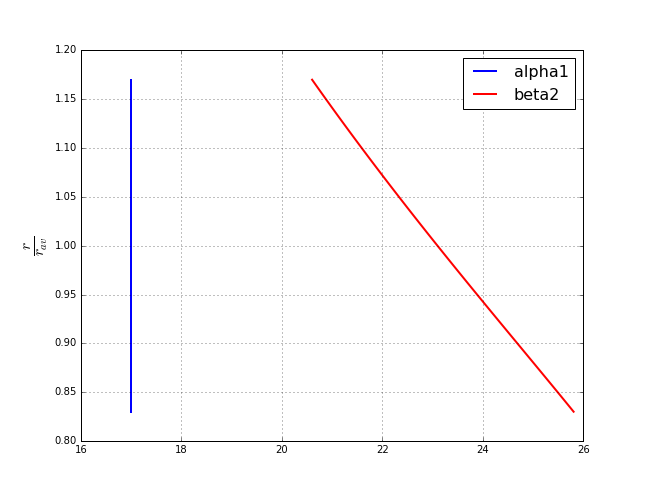
\includegraphics[scale=0.3]{../../plots/alpha1_beta2_st1.png}
\caption{Изменение углов $\alpha_1$ и $\beta_2$ по радиусу}
\end{figure}

\begin{figure}[hbtp]
\centering
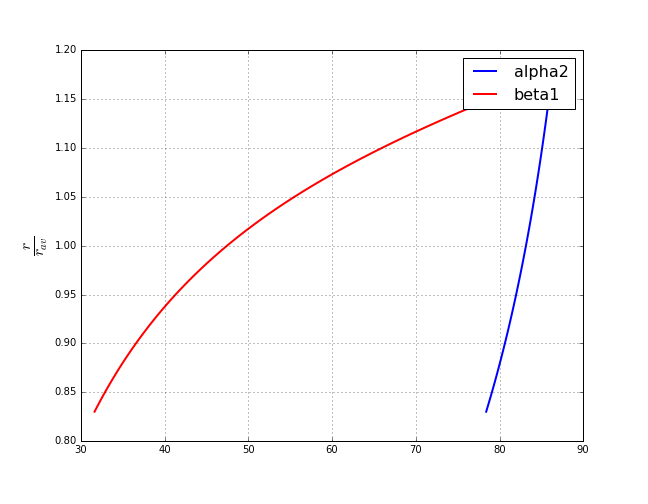
\includegraphics[scale=0.3]{../../plots/alpha2_beta1_st1.png}
\caption{Изменеие углов $\alpha_2$ и $\beta_1$ по радиусу}
\end{figure}

\begin{figure}[hbtp]
\centering
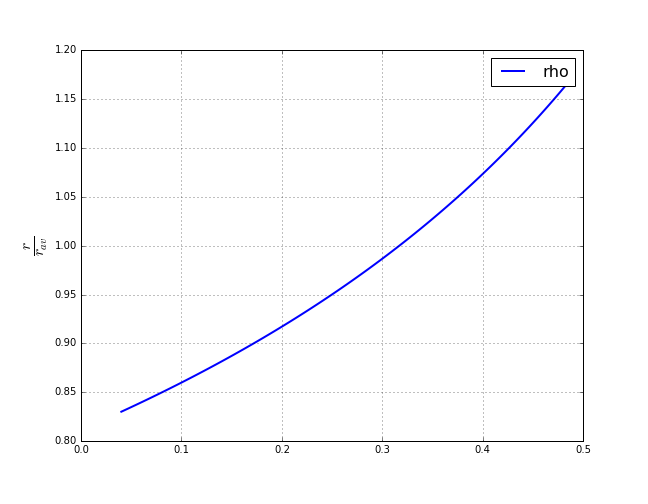
\includegraphics[scale=0.3]{../../plots/rho_st1.png}
\caption{Изменение степени реактивности по радиусу}
\end{figure}

\begin{figure}[hbtp]
\centering
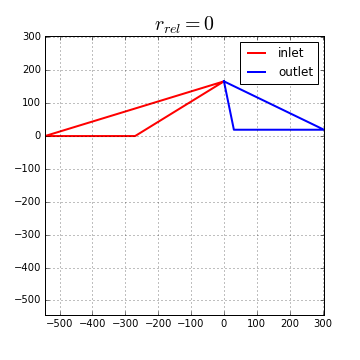
\includegraphics[scale=0.5]{../../plots/st1_triangles_0.png}
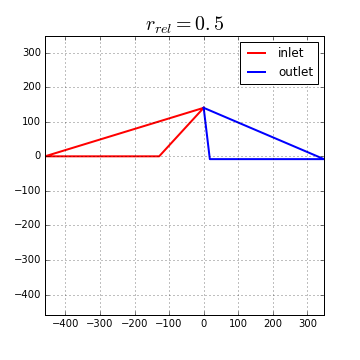
\includegraphics[scale=0.5]{../../plots/st1_triangles_1.png}
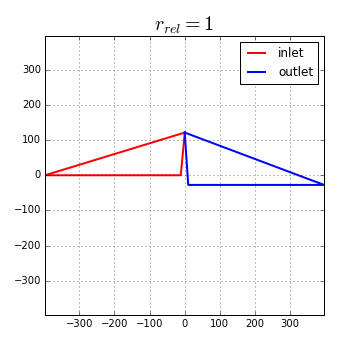
\includegraphics[scale=0.5]{../../plots/st1_triangles_2.png}
\caption{Треугольники скоростей}
\end{figure}


\section{Расчет на прочность диска первой ступени}
\subsection{Исходные данные для расчета}
\begin{enumerate}
\item Частота вращения: $n = 18000.0\ об/мин$
\item Зависимость толщины диска от радиуса: $h\left( r \right)$
\item Сила инерции, действующая на лопатку: $P_{лоп} = 39960.0\ Н$
\item Ширина хвостовика: $h_{m-1} = 0.01587\ м$
\item Радиусы хвостовика: $r1 = 0.12786\ м$ и $r2 = 0.13864\ м$
\item Температура на внутреннем радиусе: $T_1 = 200\ К$
\item Температура на внешенм радиусе: $T_m = 700\ К$
\item Закон изменения температуры диска по радиусу: 
Примем, что температура диска изменяется по радиусу по закону квадратной параболы:
\[T\left( r \right) = T_1 + \left( T_m - T_1 \right) \frac{r}{r_m} ^2\]
\item Число лопаток: $z_{л} = 48$
\item Параметры материала:

\begin{enumerate}
	\item Материал - сплав ЭИ698.
	\item Плотность: $\rho = 8320 кг/м^3$
	\item Коэффициент Пуассона: $\mu = 0.3$
	\item Зависимость модуля Юнга от температуры:
	
	\begin{tabular}{|c|c|c|c|c|c|c|}
	\hline 
	T, К & 20 & 400 & 500 & 600 & 700 & 800 \\ 
	\hline 
	E, МПа & $2\cdot10^5$ & $1.82\cdot10^5$ & $1.75\cdot10^5$ & $1.65\cdot10^5$ & $1.55\cdot10^5$ & $1.4\cdot10^5$ \\ 
	\hline 
	\end{tabular} 
	
	\item Зависимость коэффициента линейного раширения от температруы
	
	\begin{tabular}{|c|c|c|c|c|c|c|c|c|c|}
	\hline 
	T, К & 100 & 200 & 300 & 400 & 500 & 600 & 700 & 800 & 900 \\ 
	\hline 
	$\alpha, 10^{-6} 1/К$ & 11 & 11.4 & 11.7 & 12.1 & 12.4 & 12.7 & 13.4 & 13.9 & 14.7 \\ 
	\hline 
	\end{tabular} 
	
	\item Зависимость предела временной прочности от температуры
	
	\begin{tabular}{|c|c|c|c|c|c|}
		\hline 
		T, К & 20 & 400 & 500 & 600 & 700 \\ 
		\hline 
		$\sigma_в, МПа$ & 1220 & 1180 & 1160 & 1120 & 1040 \\ 
		\hline 
		\end{tabular} 	
	
\end{enumerate}
\end{enumerate}

\subsection{Алгоритм расчета}
\begin{enumerate}
\item Определяем силу нагрузку на периферии:
\[p_m = \frac{P_{лоп} z_{л}}{2 \pi r_{2} h_{m-1}} + 
  \rho \left( \frac{\pi n}{30} \right)^2 \frac{r_2^3 - r_1^3}{3 r_1} = 
  \frac{39960.0 \cdot 48}{2 \pi  \cdot 0.13864 \cdot 0.01587} + 
  8320 \cdot \left( \frac{\pi \cdot 18000.0}{30} \right)^2 \frac{ 0.13864^3 -  0.12786^3}{3  0.12786} = 198.13\ МПа\]
 \item Разобьем диск на $m-1$ участков постоянной толщины.
 \item Зададим значение $\sigma_r^{1,1} = \sigma_t^{1,1}=100..200\ МПа$
 \item Длякаждого из участков решим следующую систему уравнений:
 \begin{equation*}
 \begin{cases}
 S_{i,i} = \sigma_r^{i,i} + \sigma_t^{i,i}, 
 \\
 D_{i,i} = \sigma_r^{i, i} - \sigma_t^{i,i},
 \\
 S_{i,i+1} =  S_{i,i} - \frac{1+ \mu}{2}\rho_i \omega^2 
 \left( r_{i+1}^2 - r_i^2 \right) - E_i \left( \theta_{i+1} - \theta_i \right),
 \\
  D_{i, i+1} = D_{i, i} \frac{r_i^2}{r_{i+1}^2} + \frac{1- \mu}{4} \rho \omega^2 \left( r_{i+1} ^2 - \frac{r_i^4}{r_{i+1}^2} \right) + 
  2 \frac{E_i}{r_{i+1}^2} \int\limits_{r_i}^{r_{i+1}}\theta r dr - E_{i} \left(
  \theta_{i+1} - \theta_i \frac{r_i^2}{r_{i+1}^2} \right),
  \\
\sigma_t^{i, i+1} = \frac{S_{i,i+1} + D_{i,i+1}}{2},
\\
\sigma_r^{i, i+1} = \frac{S_{i,i+1} - D_{i,i+1}}{2},
\\
\sigma_r^{i+1, i+1} = \sigma_r^{i, i+1} \frac{h_i}{h_{i+1}},
\\
\sigma_t^{i+1, i+1} = \mu \sigma_t^{i, i+1} \frac{h_i}{h_{i+1}} + 
\frac{E_{i+1}}{E_i} \left(\sigma_t^{i,i+1} - \mu \sigma_r^{i, i+1} \right),
 \end{cases} 
 \end{equation*}
 где $\theta \left( r_i \right) = \alpha \left( r_i \right)  
 \left( T\left( r_i \right) - T_0 \right)$ - температурные деформации, а $T_0 = 20^\circ C$
 \item Повторяем пукты 3 и 4 при $\theta=0$ и $\omega = 0$
 \item Находим коэффициент $k$:
 \[k = \frac{p_m - (\sigma_r^{m-1, m})_I}{(\sigma_r^{m-1, m})_{II}}\]
 \item Находим значения напряжений на каждом из участков:
 \[\sigma_r^{i,j} = (\sigma_r^{i,j})_I + k(\sigma_r^{m-1, m})_{II}\]
 \[\sigma_t^{i,j} = (\sigma_t^{i,j})_I + k(\sigma_t^{m-1, m})_{II}\]
\end{enumerate}

\subsection{Результаты расчета}
\begin{enumerate}

\item Результаты первого расчета.

\begin{center}
\begin{tabular}{|c|c|c|c|}
\hline 
$i$ & $r_i,\ мм$ & $\sigma_r^{i,j},\ МПа$ & $\sigma_t^{i,j},\ МПа$ \\ 
\hline 

0 & 0.0 & 100.0 & 100.0 \\ \hline 0 & 6.3 & 98.8 & 97.6 \\ \hline 1 & 6.3 & 101.5 & 98.4 \\ \hline 1 & 12.7 & 97.2 & 91.8 \\ \hline 2 & 12.7 & 100.0 & 92.6 \\ \hline 2 & 19.0 & 93.2 & 81.1 \\ \hline 3 & 19.0 & 96.0 & 81.8 \\ \hline 3 & 25.4 & 86.8 & 65.5 \\ \hline 4 & 25.4 & 89.5 & 66.2 \\ \hline 4 & 31.7 & 77.9 & 44.8 \\ \hline 5 & 31.7 & 80.3 & 45.5 \\ \hline 5 & 38.1 & 66.4 & 19.1 \\ \hline 6 & 38.1 & 68.5 & 19.8 \\ \hline 6 & 44.4 & 52.2 & -11.6 \\ \hline 7 & 44.4 & 53.9 & -11.0 \\ \hline 7 & 50.7 & 35.2 & -47.6 \\ \hline 8 & 50.7 & 36.1 & -47.1 \\ \hline 8 & 57.1 & 15.1 & -89.0 \\ \hline 9 & 57.1 & 15.4 & -88.4 \\ \hline 9 & 63.4 & -8.1 & -136.9 \\ \hline 10 & 63.4 & -8.3 & -136.1 \\ \hline 10 & 69.8 & -34.3 & -190.3 \\ \hline 11 & 69.8 & -35.1 & -189.4 \\ \hline 11 & 76.1 & -63.5 & -249.4 \\ \hline 12 & 76.1 & -65.9 & -248.4 \\ \hline 12 & 82.5 & -96.8 & -313.8 \\ \hline 13 & 82.5 & -100.6 & -312.2 \\ \hline 13 & 88.8 & -133.6 & -382.0 \\ \hline 14 & 88.8 & -139.1 & -379.2 \\ \hline 14 & 95.1 & -174.3 & -454.8 \\ \hline 15 & 95.1 & -181.7 & -451.3 \\ \hline 15 & 101.5 & -218.9 & -532.6 \\ \hline 16 & 101.5 & -228.6 & -526.8 \\ \hline 16 & 107.8 & -267.8 & -613.7 \\ \hline 17 & 107.8 & -280.2 & -604.7 \\ \hline 17 & 114.2 & -321.0 & -698.9 \\ \hline 18 & 114.2 & -336.7 & -688.0 \\ \hline 18 & 120.5 & -379.7 & -804.1 \\ \hline 19 & 120.5 & -294.2 & -759.1 \\ \hline 19 & 126.9 & -343.0 & -879.3 \\ \hline 
\end{tabular} 
\end{center}

\item Результаты второго расчета

\begin{center}
\begin{tabular}{|c|c|c|c|}
\hline 
$i$ & $r_i,\ мм$ & $\sigma_r^{i,j},\ МПа$ & $\sigma_t^{i,j},\ МПа$ \\ 
\hline 

0 & 0.000000 & 100.000000 & 100.000000 \\ \hline 0 & 6.300000 & 100.000000 & 100.000000 \\ \hline 1 & 6.300000 & 102.800000 & 100.800000 \\ \hline 1 & 12.700000 & 102.000000 & 101.500000 \\ \hline 2 & 12.700000 & 104.900000 & 102.300000 \\ \hline 2 & 19.000000 & 104.200000 & 103.100000 \\ \hline 3 & 19.000000 & 107.300000 & 103.900000 \\ \hline 3 & 25.400000 & 106.500000 & 104.600000 \\ \hline 4 & 25.400000 & 109.700000 & 105.400000 \\ \hline 4 & 31.700000 & 109.000000 & 106.200000 \\ \hline 5 & 31.700000 & 112.400000 & 107.000000 \\ \hline 5 & 38.100000 & 111.500000 & 107.800000 \\ \hline 6 & 38.100000 & 115.100000 & 108.700000 \\ \hline 6 & 44.400000 & 114.300000 & 109.500000 \\ \hline 7 & 44.400000 & 118.100000 & 110.300000 \\ \hline 7 & 50.700000 & 117.200000 & 111.200000 \\ \hline 8 & 50.700000 & 120.300000 & 111.800000 \\ \hline 8 & 57.100000 & 119.400000 & 112.700000 \\ \hline 9 & 57.100000 & 121.900000 & 113.100000 \\ \hline 9 & 63.400000 & 121.100000 & 113.900000 \\ \hline 10 & 63.400000 & 123.700000 & 114.200000 \\ \hline 10 & 69.800000 & 122.900000 & 115.000000 \\ \hline 11 & 69.800000 & 125.800000 & 115.400000 \\ \hline 11 & 76.100000 & 125.000000 & 116.200000 \\ \hline 12 & 76.100000 & 129.700000 & 117.100000 \\ \hline 12 & 82.500000 & 128.800000 & 118.000000 \\ \hline 13 & 82.500000 & 133.800000 & 118.800000 \\ \hline 13 & 88.800000 & 132.800000 & 119.800000 \\ \hline 14 & 88.800000 & 138.200000 & 120.400000 \\ \hline 14 & 95.100000 & 137.100000 & 121.500000 \\ \hline 15 & 95.100000 & 142.900000 & 122.200000 \\ \hline 15 & 101.500000 & 141.700000 & 123.400000 \\ \hline 16 & 101.500000 & 148.000000 & 123.800000 \\ \hline 16 & 107.800000 & 146.600000 & 125.200000 \\ \hline 17 & 107.800000 & 153.400000 & 125.300000 \\ \hline 17 & 114.200000 & 151.900000 & 126.800000 \\ \hline 18 & 114.200000 & 159.300000 & 126.900000 \\ \hline 18 & 120.500000 & 157.700000 & 128.600000 \\ \hline 19 & 120.500000 & 122.200000 & 115.700000 \\ \hline 19 & 126.900000 & 121.900000 & 116.000000 \\ \hline 
\end{tabular} 
\end{center}

\item Значение коэффициента $k$:
\[k = \frac{p_m - (\sigma_r^{m-1, m})_I}{(\sigma_r^{m-1, m})_{II}} = 
\frac{198.13 - -343.03}{121.861} = 4.4408\]

\item Значения напряжений на участках после пересчета.

\begin{center}
\begin{tabular}{|c|c|c|c|}
\hline 
$i$ & $r_i,\ мм$ & $\sigma_r^{i,j},\ МПа$ & $\sigma_t^{i,j},\ МПа$ \\ 
\hline 

0 & 0.000000 & 544.100000 & 544.100000 \\ \hline 0 & 6.300000 & 542.900000 & 542.900000 \\ \hline 1 & 6.300000 & 557.900000 & 546.000000 \\ \hline 1 & 12.700000 & 550.300000 & 550.300000 \\ \hline 2 & 12.700000 & 566.000000 & 547.100000 \\ \hline 2 & 19.000000 & 556.100000 & 556.100000 \\ \hline 3 & 19.000000 & 572.300000 & 543.100000 \\ \hline 3 & 25.400000 & 559.900000 & 559.900000 \\ \hline 4 & 25.400000 & 576.800000 & 534.300000 \\ \hline 4 & 31.700000 & 561.800000 & 561.800000 \\ \hline 5 & 31.700000 & 579.300000 & 520.700000 \\ \hline 5 & 38.100000 & 561.700000 & 561.700000 \\ \hline 6 & 38.100000 & 579.800000 & 502.300000 \\ \hline 6 & 44.400000 & 559.600000 & 559.600000 \\ \hline 7 & 44.400000 & 578.200000 & 479.000000 \\ \hline 7 & 50.700000 & 555.500000 & 555.500000 \\ \hline 8 & 50.700000 & 570.200000 & 449.500000 \\ \hline 8 & 57.100000 & 545.200000 & 545.200000 \\ \hline 9 & 57.100000 & 556.700000 & 413.700000 \\ \hline 9 & 63.400000 & 529.500000 & 529.500000 \\ \hline 10 & 63.400000 & 540.900000 & 371.100000 \\ \hline 10 & 69.800000 & 511.300000 & 511.300000 \\ \hline 11 & 69.800000 & 523.700000 & 323.100000 \\ \hline 11 & 76.100000 & 491.600000 & 491.600000 \\ \hline 12 & 76.100000 & 510.100000 & 271.400000 \\ \hline 12 & 82.500000 & 475.100000 & 475.100000 \\ \hline 13 & 82.500000 & 493.800000 & 215.200000 \\ \hline 13 & 88.800000 & 456.100000 & 456.100000 \\ \hline 14 & 88.800000 & 474.800000 & 155.400000 \\ \hline 14 & 95.100000 & 434.500000 & 434.500000 \\ \hline 15 & 95.100000 & 453.000000 & 91.200000 \\ \hline 15 & 101.500000 & 410.200000 & 410.200000 \\ \hline 16 & 101.500000 & 428.500000 & 22.900000 \\ \hline 16 & 107.800000 & 383.200000 & 383.200000 \\ \hline 17 & 107.800000 & 401.100000 & -48.400000 \\ \hline 17 & 114.200000 & 353.500000 & 353.500000 \\ \hline 18 & 114.200000 & 370.800000 & -124.300000 \\ \hline 18 & 120.500000 & 320.500000 & 320.500000 \\ \hline 19 & 120.500000 & 248.400000 & -245.500000 \\ \hline 19 & 126.900000 & 198.100000 & 198.100000 \\ \hline 
\end{tabular} 
\end{center}

\item Средние арифметические значения напряжений на радиусах

\begin{center}
\begin{tabular}{|c|c|c|c|c|}
\hline 
$i$ & $r_i,\ мм$ & $\sigma_r^{i},\ МПа$ & $\sigma_t^{i},\ МПа$ & $\sigma_{экв}^i$ \\ 
\hline 
0 & 0.000000 & 544.100000 & 544.100000 & 544.100000 \\ \hline 1 & 6.300000 & 550.400000 & 543.900000 & 550.400000 \\ \hline 2 & 12.700000 & 558.100000 & 544.900000 & 558.100000 \\ \hline 3 & 19.000000 & 564.200000 & 541.000000 & 564.200000 \\ \hline 4 & 25.400000 & 568.400000 & 532.200000 & 568.400000 \\ \hline 5 & 31.700000 & 570.600000 & 518.600000 & 570.600000 \\ \hline 6 & 38.100000 & 570.800000 & 500.100000 & 570.800000 \\ \hline 7 & 44.400000 & 568.900000 & 476.800000 & 568.900000 \\ \hline 8 & 50.700000 & 562.800000 & 448.000000 & 562.800000 \\ \hline 9 & 57.100000 & 551.000000 & 412.600000 & 551.000000 \\ \hline 10 & 63.400000 & 535.200000 & 370.000000 & 535.200000 \\ \hline 11 & 69.800000 & 517.500000 & 321.800000 & 517.500000 \\ \hline 12 & 76.100000 & 500.800000 & 269.100000 & 500.800000 \\ \hline 13 & 82.500000 & 484.500000 & 212.700000 & 484.500000 \\ \hline 14 & 88.800000 & 465.500000 & 152.700000 & 465.500000 \\ \hline 15 & 95.100000 & 443.800000 & 88.100000 & 443.800000 \\ \hline 16 & 101.500000 & 419.300000 & 19.200000 & 419.300000 \\ \hline 17 & 107.800000 & 392.200000 & -53.100000 & 421.200000 \\ \hline 18 & 114.200000 & 362.200000 & -130.000000 & 441.800000 \\ \hline 19 & 120.500000 & 284.400000 & -239.300000 & 454.200000 \\ \hline 
\end{tabular} 
\end{center}

\item Максимальная величина эквивалентных напряжений:
\[\sigma_{экв}^i = \sqrt{(\sigma_1^i)^2 + (\sigma_3^i)^2 - \sigma_1^i \sigma_3^i}\]
\[\sigma_{экв\ мах} = 570.773\ МПа\]
\item Минимальный коэффициент запаса по временной прочности:
\[n_{в min} = 2.096\]
\item Коэффициенты концентраций напряжений у отверстий:
\[k_1 = 3 - \frac{d_1}{b_1} - \frac{\sigma_{r1}}{\sigma_{t1}} = 
3 - \frac{0.0085}{0.0255} - \frac{537.52}{376.231} = 1.238\]
\[k_2 = 3 - \frac{d_2}{b_2} - \frac{\sigma_{r2}}{\sigma_{t2}} = 
3 - \frac{0.005}{0.023} - \frac{562.983}{448.628} = 1.516\]
\item Напряжения в зонах концентрации:
\[\sigma_{tк1} = k_1 \sigma_{t1} = 1.238 \cdot 376.231 = 465.763\]
\[\sigma_{tк2} = k_2 \sigma_{t2} = 1.516 \cdot 448.628 = 671.327\]
\item Зависимотb от радиуса радиальных, окружных и эквивалентных напряжений, а также коэффициента запаса по временной прочности.
\begin{figure}[hbtp]
\centering
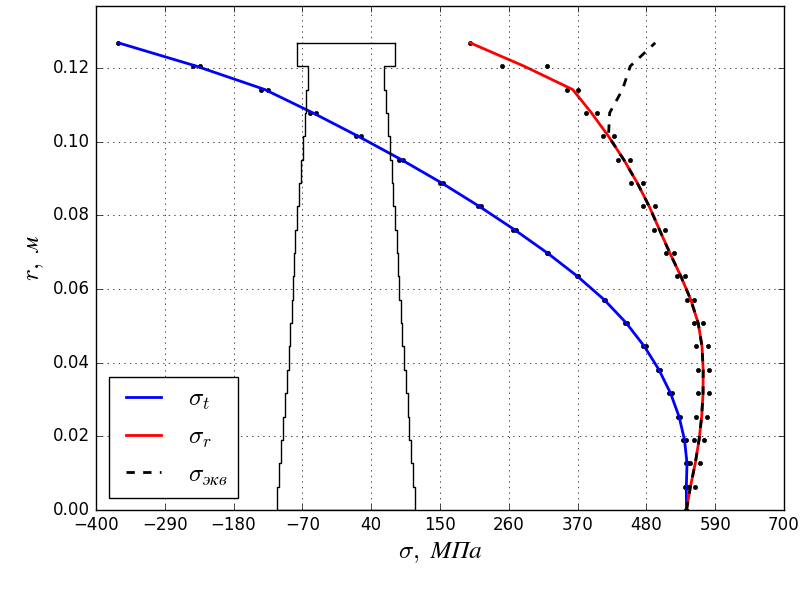
\includegraphics[scale=0.7]{../../strength_calculation/output/StressPlot.png}
\caption{Зависимость напряжений от радиуса}
\end{figure}
\begin{figure}[hbtp]
\centering
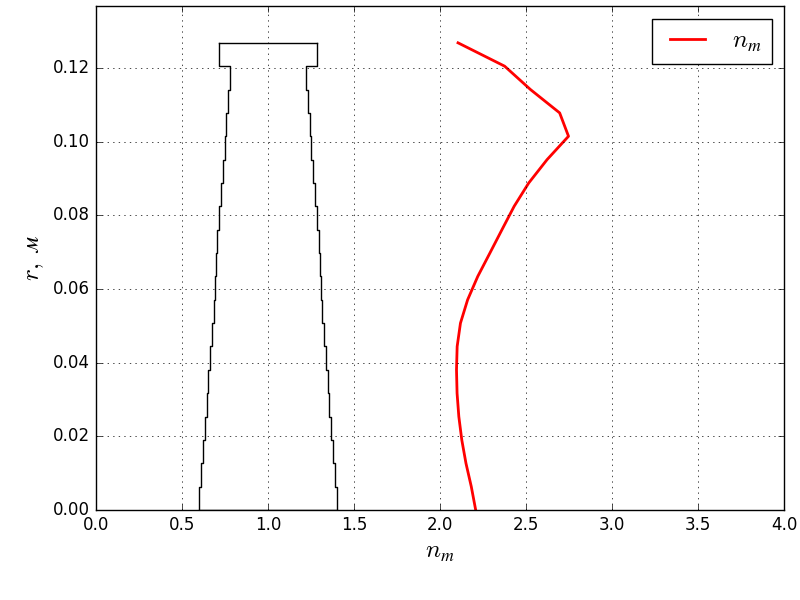
\includegraphics[scale=0.7]{../../strength_calculation/output/SafetyFactorPlot.png}
\caption{Зависимость коэффициента запаса от радиуса}
\end{figure}

\end{enumerate}
\end{document}
